%%%%%%%%%%%%%%%%%%%%%%%%%%%%%%%%
% SECTION :: IR in our project %
%%%%%%%%%%%%%%%%%%%%%%%%%%%%%%%%
\section{IR in our project}
%%%%%%%%%%%%%%%%%%%%%%%%%%%%%%%%%%%
% Frame Open :: IR in our project %
%%%%%%%%%%%%%%%%%%%%%%%%%%%%%%%%%%%
\frame{\frametitle{IR in our project :: Overflow handled in IR $\rightarrow$ MIPS}
\begin{figure}[htbp]
\begin{center}
% Requires \usepackage{graphicx}
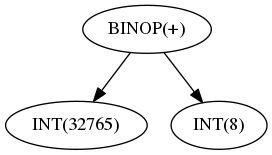
\includegraphics[width=4.0cm]{AST.png}\\
\label{Figure_Simple_Addition_Of_2_Integers_AST}
\end{center}
\end{figure}
\begin{itemize}
\item Handling arithmetic overflow in the IR $\rightarrow$ MIPS phase
      will yield the following (simple) IR code for the addition above:
%%%%%%%%%%%%%%%%%%
% Table :: Begin %
%%%%%%%%%%%%%%%%%%
\begin{table}[h]
\centering
\begin{tabular}{ l }
%%%%%%%%%%%%%%%%%%%%%%%%%%%%%%%%%
                               \\
li Temp\_24, 32765             \\
li Temp\_25, 8                 \\
add Temp\_23,Temp\_24,Temp\_25 \\
%%%%%%%%%%%%%%%%%%%%%%%%%%%%%%%%%
\end{tabular}
\caption*{\label{Table_Leaving_Overflow_To_IR_2_MIPS}}
\end{table}
\item What is the benefit of a simpler IR?
      How will the add instruction be translated to MIPS eventually?
\end{itemize}

%%%%%%%%%%%%%%%%%%%%%%%%%%%%%%%%%%%
% Frame Close :: Warm up examples %
%%%%%%%%%%%%%%%%%%%%%%%%%%%%%%%%%%%
}